\documentclass[letterpaper, 10pt,titlepage]{article}

\usepackage[utf8]{inputenc}
\usepackage [english]{babel}
\usepackage [autostyle, english = american]{csquotes}
\usepackage{graphicx}
\usepackage{amssymb}                                         
\usepackage{amsmath}                                         
\usepackage{amsthm}                                          
\usepackage{alltt}                                           
\usepackage{float}
\usepackage{color}
\usepackage{url}
\newcommand\tab[1][1cm]{\hspace*{#1}}
\setlength{\parindent}{0em}
\setlength{\parskip}{1em}
\usepackage{pst-gantt}
\usepackage{pst-tools}
\usepackage[letterpaper, margin=0.75in]{geometry}
\usepackage[TABBOTCAP, tight]{subfig}
\usepackage{balance}
\usepackage{enumitem}
\usepackage{hyperref}
\hypersetup{
  colorlinks = true,
  linkcolor  = black
}

\setcounter{secnumdepth}{4}
\def\name{Group 48}

\graphicspath{ {images/}}

\hypersetup{
  colorlinks = true,
  urlcolor = black,
  pdfauthor = {\name},
  pdfkeywords = {The Preliminary Design Document},
  pdftitle = {Capstone Project},
  pdfsubject = {Capstone Project},
  pdfpagemode = UseNone
}



\begin{document}

\begin{titlepage}
\begin{center}
    \Huge
    \textbf{The Preliminary Design Document}
    \textbf{Capstone Project}\\
    \vspace{1.0cm}
    \large
    Developers: Sung Kim, Xiaoli Sun, Zijian Huang\\
    Client: David Vasquez\\
    \vspace{1.5cm}
    \large
    Instructor: D. Kevin McGrath\\

    \large
    CS 461, Fall 2017, Oregon State University\\    

    \vspace{3.2cm}

    \large
    \underline{Abstract}\\
    \vspace{0.3cm}
    \end{center}
    \large

    \tab For the Campus Event Mobile Application program, the client David Vasquez want to make life more convenient for each students, instructors or even residents live in Corvallis since there are lots of events happen everyday. A great mobile application is useful for every user and improve the quality of life. The mobile application will be developed in two forms: one developed for the Android mobile platform, and the other developed for the iOS mobile development. For the ease of development, these two forms of the mobile application will be developed with a framework called React Native which support cross platform development, they will be using the same methods of providing campus events to users. The mobile application will display current events and group events by loading data from MySQL database. In addition, the mobile application will allow users discover different events from different sections, follow and unfollow events, and edit user profile. Our team will divide this project into three sections (Notification push/Secure Login, Data storage/User interface, Scanning/Admin website) between team members as follows: Data storage/User interface: Sung Kim, Notification push/Secure Login: Xiaoli Sun, Scanning/Admin Website: Zijian Huang. This document outlines the possible technologies that will be used for each of these three development sections.  
    \vspace{0.8cm}
    \vfill
    
\begin{center}    
    Nov 30, 2017

\end{center}
\end{titlepage}


\tableofcontents
\newpage

\section{Introduction}
\subsection{Scope}
The team will be developing a mobile application that work on both Android and IOS. The user will be provided with either a list view and/or calendar of the upcoming events, a "Discover" tab to find groups they want to follow, a "Following" tab to manage users current list of groups, and finally a "Profile" tab to edit user information. The application will also provide a secure login. If the application finishes early, the team will develop an administrator website to manage group events.
\subsection{Purpose}
The purpose of the software design descriptions(SSD) is to provide information on the different technologies that will be used during the development of the application.
\subsection{Intended Audience}
This document is intended for use by a technical user that wants to recreate this project. It should serve as a guide for the organization, design, and underlying technologies within the application.
\section{Definitions, Acronyms, and Abbreviations }
\begin{table}[ht]
\begin{tabular}{| l | p{9cm} |}
\hline
\textbf{Term} & \textbf{Definition} \\ \hline
Admin / Administrator & A user with the permissions to modify and publish events for their respective group. \\ \hline
Android & A mobile operating system developed by Google to work on various smart phones and tablets.\\ \hline
Application Program Interface (API) & An interface specifying how software components can integrate with various parts of a project or external resources. \\ \hline
Database & A structured set of data that can be accessed and modified in different ways.\\ \hline
Evently & The current name for the mobile application. May change during development. \\ \hline
Events & A planned public or private occasion sponsored by certain organizations/groups. \\ \hline
IDE & Abbreviation for Integrated Development Environment \\ \hline
iOS & A mobile operating system developed by Apple for use in their Ipod touches, Iphones, and Ipads \\ \hline
Mobile Application & A type of application software designed to run on mobile devices such as a smartphone. \\ \hline
LTS & Abbreviation for Long-term Support \\ \hline
MySQL & An open source relational database management system based on Structured Query Language(SQL) \\ \hline
Structured Query Language (SQL) & A standard language for storing, manipulating and retrieving information from a database. \\ \hline
User & Any person, or robot, that wants to make use of the mobile application. \\ \hline
\end{tabular}
\end{table}                                                


%\subsection{References}
%\vspace{0.3cm}

\section{Overall Description}
The Oregon State University community is filled with various organizations that hosts multiple events every year. These events can range from large public events such as Football games to smaller career related events such as the Oregon State Fall Career Expo. To expand the number of participants and to get the Corvallis community more involved, Evently will host multiple group events to be displayed to the public. The mobile application will display an interactive calender that will provide the users a way to keep track of all the events they want to see. Also, the users will have access to discover new groups that they can follow and participate with. To ensure user privacy, a secure login will be implemented. This application will reach out to anyone in the Corvallis community looking for something to do. Development of this application will start during Oregon States Universities Winter term, while the developers are taking classes. The time frame to complete this application is approximately three months. Since Evently is not a native OSU application, it will not be branded with the OSU logo. To ensure the application reaches a large audience, Evently will be available for both Android and IOS.

\section{Body}
\subsection{Design viewpoint: Development Environment}
\subsubsection{JavaScript}
Our project will be released for both Android and iOS version. For Android and iOS development, the language that we choose will mainly based on whether it could be implemented cross platform or not. Since we will develop our project in React Native, JavaScript will be a perfect solution. Unlike Java, if a developer wants to build apps use JavaScript, a native WebView wrapper should be created first. A JavascriptAdapter with some JavaScript method in it allow users access the application. Moreover, a framework like Appcelerator or PhoneGap is popular to use when a developer tries to write an app in Android using JavaScript. In our project, we will write JavaScript code for our project and then using a tool called React Native to convert the code to Android and iOS version. 

Although the application written by JavaScript runs the slowest among Java, JavaScript and C/C++, We still choose JavaScript because JavaScript not only support the same APIs as Java, but also support cross platform implementation which could decrease the difficulties and time for developing the product. It also doesn't contain secure issue like memory leak exist in C/C++.

\subsubsection{React Native}

To meet our original requirement of having an application for both Android and iOS, we came to the conclusion of developing the application in the React Native Framework. React native is based off the React JavaScript Library, so using an IDE compatible with JavaScript is a must. 

A good option would be to grab the Atom IDE. Atom is a open-source IDE that's highly customizable when writing JavaScript applications. Another requirement to use React Native, would be to install NodeJS. We will download the latest LTS version, which is recommended for most users. NodeJS provides us with NPM which is a package manager that will help us install React Native. 

To test our code, React Native has the Expo Client. This is a mobile application that can be downloaded from the App Store and Google Play. Expo will scan a QR code, that's created after compiling your JavaScript code, and will run the application on your personal device. 

\subsection{Design viewpoint: Functionality}
\subsubsection{Secure Login}
Account information security is always a big issue in application development. With some good secure login technology, user’s personal information will have a more complete protection. We plan to implement oAuth 2.0 as secure login in our project. 

The basic OAuth 2.0 protocol flow is showed as below: 
\begin{enumerate}
\item Users will be asked to enter user name and password before login. 
\item After users enter user name and password, the application will receive an authorization grant and begin to request an access token from server. 
\item If the application identity and authorization grant is valid, API server will issue an access token. 
\item The application then could use the access token to request information from API server. 
\item If the access token is valid, the application will retrieve information from server as JSON strings.
\end{enumerate}
Moreover, the application must be registered to the service’s website before using OAuth 2.0. For example, if a developer wants to develop an application with a function like “Sign in with Twitter”, he needs to create an application in https://apps.twitter.com/. Once the application is successfully created, the developer will get a consumer key (API key) and consumer secret (API secret). The consumer key is used to build authorization URLs.  When a user’s account is accessed, the consumer secret is used to identify the application to service API. Authorization grant has four types: authorization code, implicit, resource owner password credentials and client credentials.\cite{OAuth2}

For implementing this function in our application, I will first use an React Native API called linking which allow me to build an interface to interact both incoming and outgoing application links. After that, I will register our application with OSU. Once the application is registered, setup a redirect URL corresponding to the URL scheme. Then add the application key to the configuration file in the application. Finally, I will show user the OSU Oauth authentication page on OSU website. For Android, I can directly call navigate method to pass the url. For iOS, I need to add an event listener to call handleOpenUrl for incoming link.

\subsubsection{Notification push}
Notification push is a very important function in our project. If this function works perfectly, users will get upcoming events' notification on time and no need to worry about missing them.

Firebase Cloud Messaging(FCM) is a new version of Google Cloud messaging. Developers are allowed to send two types of messages: notification messages and data messages. For sending notification message, developers could use Admin SDK or the FCM Server Protocols to set the notification key first, and then use the notifications composer to build the content and send it to users. For data message, developers could use the Admin SDK or the Server Protocols to set the data key only because data messages will be processed by application itself. When the application is in the background, the notification will be sent to the notification tray. When in forground, onMessageReceived() funtion could be used to process messages. Data message will be received by using the function onMessageReceived() as well.\cite{firebasecloudmessage}

Comparing to other notification push method, FCM not only provide local and scheduled notification push, but also support user to user messaging. It also contains Firebase Notifications (which is a web console) so that it's convenient for developers to test the function in the console. Some new client side features also support FCM SDK only.

For implementing FCM on our application, I will first use this library: react-native-fcm. First of all, I will install and configure this library. Installation is quite simple, I only need to use this command: ``react-native link react-native-fcm''. The next step is to configure Firebase console for both Android and iOS. For Android configuration, I need to edit build.gradle under both android folder, project/app, and android/app folder. AndroidManifest.xml under android/app/src/main will alos need to be modified. Then I will define activities on intent. For iOS configuration, I will install a dependency manager called CocoaPods then initialize Pods by using this command: ``cd ios \&\& pod init''. The next step is to edit Podfile and install Firebase pod by using ``pod install'' command. After that, I will configure FCM APN by uploading the authentication key from Apple Developer account and a provisioning file for the Application ID. Then I can edit AppDelegate.h/AppDelegate.m and setup XCode build. Finally, I will configure FCM by getting google-services.json and GoogleService-Info.plist from FCM console and put these two files to specific folder.

\subsection{Design viewpoint: Data Storage}

\subsubsection{MySQL}
To properly manage all the data we receive, we need to store it in a secure location. We looked into various solutions for this issue and came across relational and NoSQL databases. NoSQL databases are not as secure as relational, so we looked into options in this category. Of the relational databases, we looked into MySQL was the best for this project.

In the current stage of the application, we need around four tables. These tables will hold information about the user, group administrators, the groups themselves and the events they will be hosting. The "user" table will store information such as a unique user pin, information based on their interests, and maybe user profile pictures. The group admin table will be used to store administrator information like the groups they manage. The group's table will store information that will be displayed on the discovery tab and within the events table, information such as location and time. These tables will have proper primary and foreign key relationships for ease of access when using the join functionality. For example, we will join together the groups and events table to display only necessary information for a user. Searching through these tables is also needed when looking through the "Discovery" tab of the application. Indexes will speed up the search process based on a row within the table. The indexes will be implemented in the group and events table.
\subsection{Design viewpoint: Interface}

\subsubsection{User Interface}

As mentioned before, the application will be developed in the React Native Framework so it can be developed for both Android and iOS. Both applications, being from the same code base, will have a similar user interface. A prototype was created using the wire framing tool Moqups. The application will be divided into fours tabs.

The "Events" tab will gather data from the database, based on the user's unique ID, and display upcoming events in either a list view or calendar view. Each event displayed will lead an events page that will hold all the information for that particular event.

  \begin{figure}[H]
	\centering
    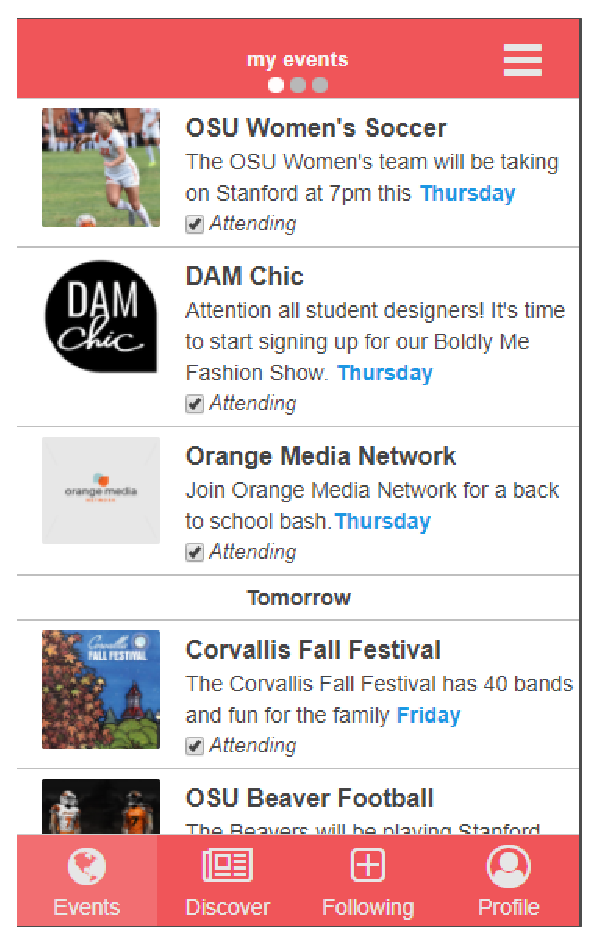
\includegraphics[scale=0.55]{events.eps}
    \captionof{figure}{Events Tab}
  \end{figure}

The "Discover" tab will lead you into a list of categories that each group is separated in. Once you've selected a category, you will be able to browse through a list of groups that host events similar to your interests. 

  \begin{figure}[H]
  \centering
    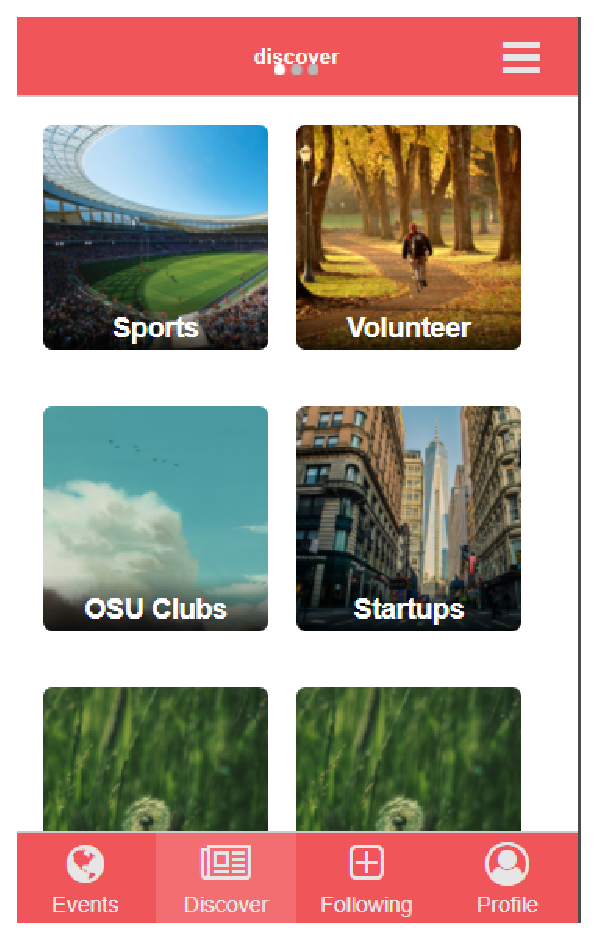
\includegraphics[scale=0.55]{discover.eps}    
    \captionof{figure}{Discover Tab}
  \end{figure}

The "Following" and "Profile" tabs gives the user the ability to manage information on their account. Data such as groups they are following and events their friends are going to.
  \begin{figure}[H]
  \centering
  \begin{minipage}{.5\textwidth}
    \centering
    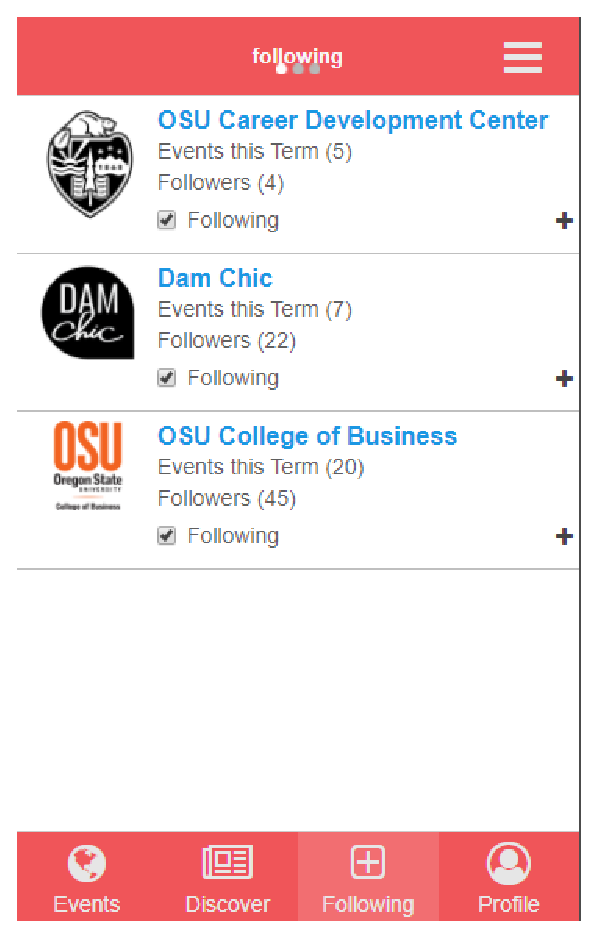
\includegraphics[width=.55\linewidth]{following.eps}
    \captionof{figure}{Following tab}
  \end{minipage}%
  \begin{minipage}{.5\textwidth}
    \centering
    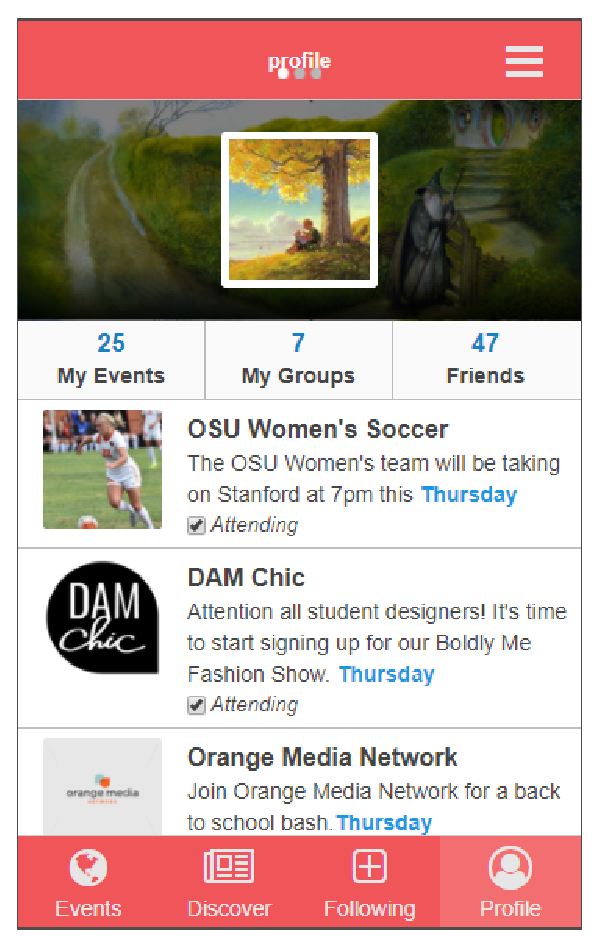
\includegraphics[width=.55\linewidth]{profile.eps}
    \captionof{figure}{Profile tab}
  \end{minipage}
  \end{figure}

\subsection{Design viewpoint: Stretch Goals}
\subsubsection{Scan function}
In some major mobile applications, using QR codes and bar codes scanner to check in or pay items. For Campus Event Mobile Application, our client David also wants to add this feature. Group 48 is going to use Mobile Vision API as the decision which we could use to build the scan function into our application if the progress of IOS and Android development are much successful than our expected. 

It is new for all group members for using Mobile Vision API. Mobile Vision API is a new computer vision algorithm which is used to develop mobile application on both IOS and Android platform. For Mobile Vision API, it has the powerful function such like FaceAPI, TextAPI and BarcodeAPI to make the mobile application which used it more useful. Considering the application we developed, we decide to use Mobile Vision API since its functional and convenient characteristic. It is helpful for develop a mobile application not only for QR code and bar code part, but also for other convenient functions we want to add in the future.

In order to achieve the development of this function, the first thing is set up an Android development environment which provided for developing Android applications on Android platform. It is easy to add functions in this environment. For IOS platform, we need to set up a related samples which distributed through CocoaPods, then we should add a file named Podfile to your Xcode project folder, if you don't have one already. After that, adding pod 'GoogleMobileVision/FaceDetector' to the Podfile. Finish all the step, running the command pod update from Terminal in the Xcode project folder. This will download and add the FaceDetector CocoaPod to the project. Finally, find the class and method descriptions for the GoogleMobileVision in the API reference to develop on IOS platform.\cite{mobilevisionapi}

\subsubsection{Website for computer browser}
It is optional to build a website for the browser user in recent popular mobile application so our group is going to design and build a website satisfying the browser user to check event.

For this plan, creating a website to be the official website of campus events mobile application or create an
application used in computer browser are two designing plan. But if we will design to create a website, HTML 5, CSS and JavaScript as the programming languages are what we need to use. 

To design for a web, programming languages shows above are tools to use. HTML 5 as a mockup language which used to create world-wide web. Almost every website are created by HTML 5 all over the world so that HTML 5 can be the foundation of the world-wide web. Every browser support HTML 5 since it is the mainstream language. We will use HTML 5 as the general framework. CSS and JavaScript are two languages which based on HTML 5 especially for CSS. CSS is a programming language which is used to add different style on HTML 5. It can change the style of word, format, form and color for HTML 5. JavaScript is a programming language which is used to make webpages interactive and provide online programs. Same as CSS, it is also a very important language of world-wide web content production. CSS and JavaScript are both used to make the web looks better and could add functions on that. PHP is a widely-used open source server-side scripting language which is suited for web development and it can be embedded into HTML5. PHP allows web developer to develop dynamic website and it is run on the server of website mostly. \cite{php} It is the language which could not be short of in development of web. Using PHP is the way to connect our web to server.

\section{Conclusion}
Campus Event Mobile Application which developed by Group 48 shows the design viewpoint above. Each of the features will suitable for every requirements for this mobile application. Also, the design must be clearly and usefully since our group is going to focus on develop this whole application step by step and make sure we are efficient and try to make no mistakes during developing. 


\section{Gantt Chart}
\newpsstyle{Important}{fillstyle=solid,fillcolor=blue}
\newpsstyle{NotImportant}{fillstyle=vlines}
\begin{center}
 
\begin{PstGanttChart}[unit=2,TaskOutsideLabelMaxSize=1, ChartShowIntervals]{14}{9} 

%------------------------ANDROID----------------------------------
\PstGanttTask[TaskInsideLabel={Android Application}]{0}{9}
\PstGanttTask[TaskOutsideLabel={Environment Set-Up},TaskUnitType=Day]{0}{6}
\PstGanttTask[TaskOutsideLabel={Calender Feature},TaskUnitType=Day]{7}{13}
\PstGanttTask[TaskOutsideLabel={Discover Feature},TaskUnitType=Day]{21}{13}
\PstGanttTask[TaskOutsideLabel={Following Feature},TaskUnitType=Day]{35}{13}
\PstGanttTask[TaskOutsideLabel={Profile Tab},TaskUnitType=Day]{49}{6}
\PstGanttTask[TaskOutsideLabel={Secure Log-in page},TaskUnitType=Day]{56}{6}
%------------------------IOS-----------------------------------
\PstGanttTask[TaskInsideLabel={iOS Application}]{0}{9}
\PstGanttTask[TaskOutsideLabel={Environment Set-Up},TaskUnitType=Day]{0}{6}
\PstGanttTask[TaskOutsideLabel={Calender Feature},TaskUnitType=Day]{7}{13}
\PstGanttTask[TaskOutsideLabel={Discover Feature},TaskUnitType=Day]{21}{13}
\PstGanttTask[TaskOutsideLabel={Following Feature},TaskUnitType=Day]{35}{13}
\PstGanttTask[TaskOutsideLabel={Profile Tab},TaskUnitType=Day]{49}{6}
\PstGanttTask[TaskOutsideLabel={Secure Log-in page},TaskUnitType=Day]{56}{6}


%\PstGanttTask[TaskStyle=Important,TaskOutsideLabel={Task 3}, TaskInsideLabel={\Large\textcolor{white}{\textbf{Important}}}]{2}{5}
%\PstGanttTask[TaskStyle=NotImportant,TaskOutsideLabel={Task 4}]{4}{2}
%\PstGanttTask[TaskOutsideLabel={Task 5}]{5}{2}

\end{PstGanttChart}
\end{center}

\newpage

\bibliography{reference,IEEEabrv}
\bibliographystyle{IEEEtran}


\end{document}
